\section{Study design}
\label{sec:study_design}
This literature study has been designed and carried out by following 
well-accepted methodological guidelines on secondary studies
\cite{petersen2015guidelines_systematic, kitchenham2013systematic_review_guidelines, wohlin2012experimentation}.

This literature study targets multiple research questions. 
These questions will be given and motivated in subsection \ref{sec:study_design:research_questions}.
Then the search and selection of papers satisfying all of the inclusion and none of the exclusion criteria began.
This process, and the criteria, are given in subsection \ref{sec:study_design:search_selection}.
After the selection was made final, hereon after called the \textit{primary studies}, 
the data extraction process began; explained in subsection \ref{sec:study_design:data_extract}. 
After data extraction, the data synthesis process began; this process is the most important step for writing the literature study. 
The studies are made comparable by finding the commonalities and patterns in the field of study. 
This process is further explained in subsection \ref{sec:study_design:data_synth}.


\subsection{Research Questions}
\label{sec:study_design:research_questions}
This study considers three research questions. These questions and their motivations are given in this subsection.

\vspace{5mm}

\textbf{[RQ1]} \textit{What are the publication trends of papers on energy efficiency in robotics software?}

\vspace{5mm}

To be able to judge any characteristics of the state-of-the-art of energy efficiency in robotics software, one needs to know the maturity of the field.
What publication trends are observed?

\vspace{5mm}

\textbf{[RQ2]} \textit{What is the state-of-the-art on analyzing and improving the energy efficiency in robotics software?}

\vspace{5mm}

This research question aims to answer what the state-of-the-art is for achieving and analyzing an increase of energy efficiency in robotics software.

\vspace{5mm}

\textbf{[RQ3]} \textit{What are the trade-offs when dealing with energy efficiency in robotics software?}

\vspace{5mm}

This research question aims to give insights into what Quality Attributes have been identified to trade-off with energy efficiency. 
It is valuable for researchers and practitioners to know that if one wants to improve energy efficiency, 
one can expect a decrease of some other attribute.

\subsection{Search and Selection}
\label{sec:study_design:search_selection}
\begin{figure}
    \centering
    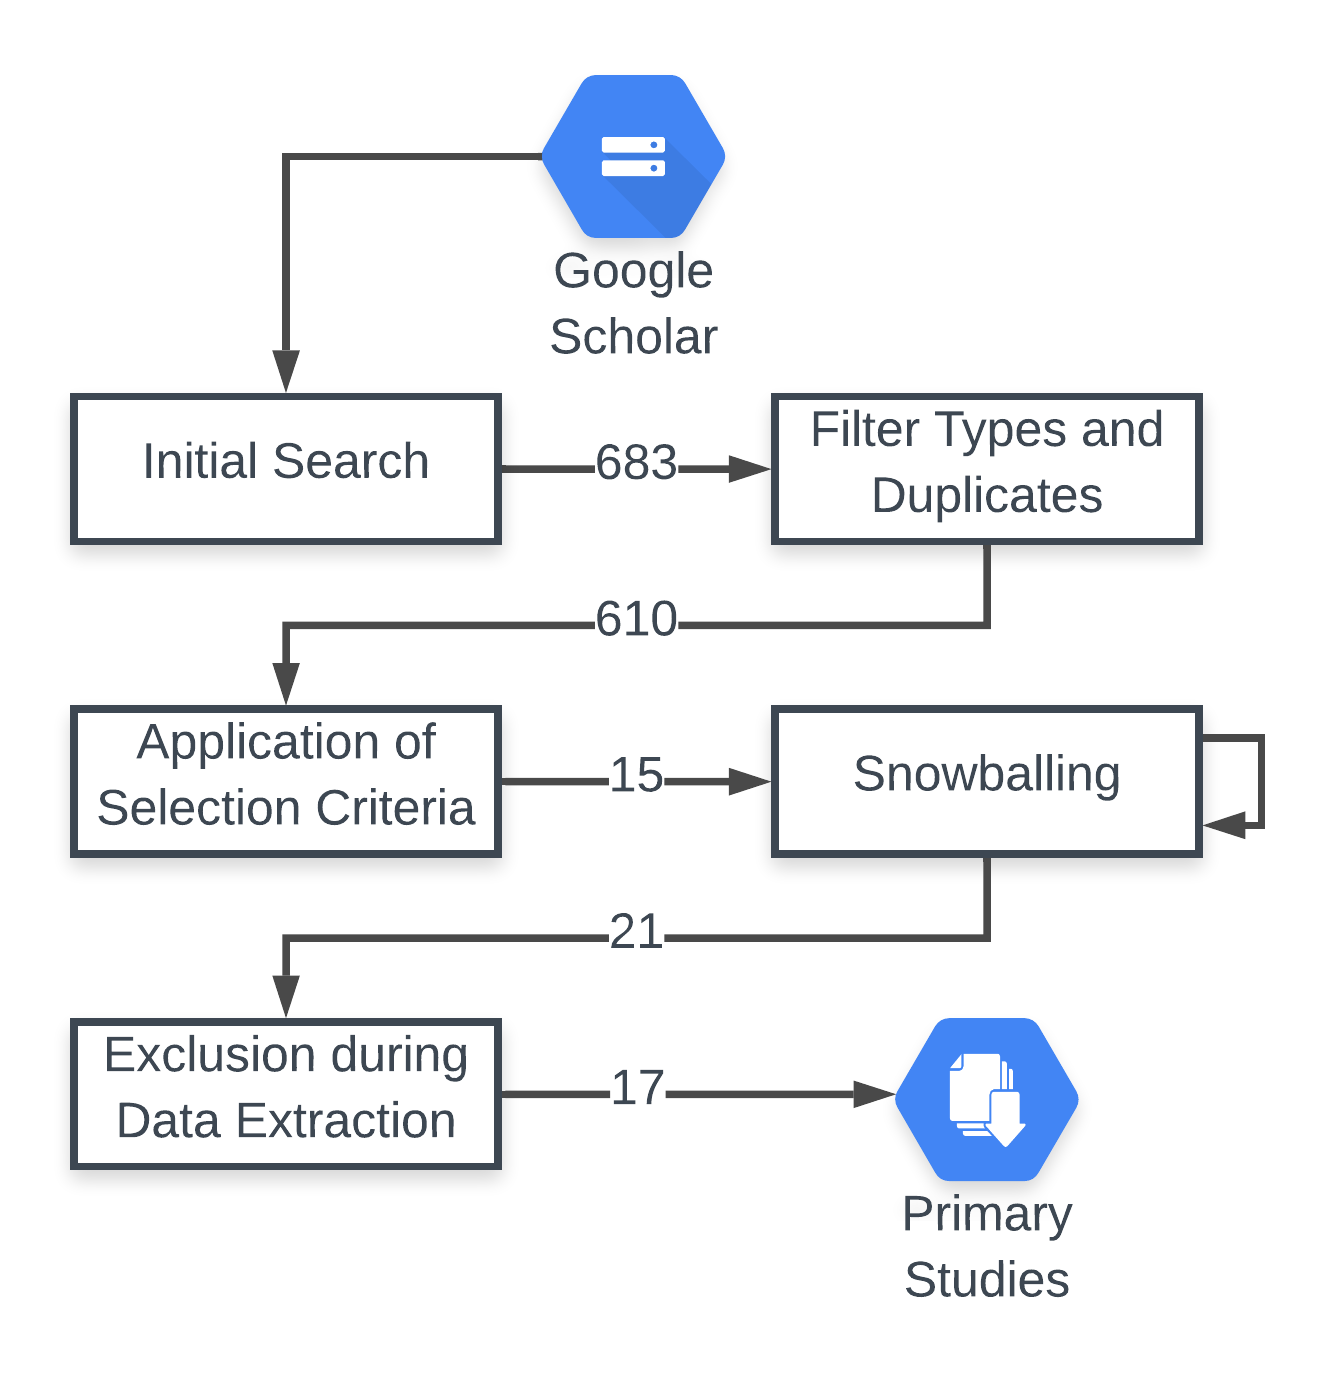
\includegraphics[width=0.5\textwidth]{figures/selection_process_var2.png}
    \caption{The search and selection process}
    \label{fig:search_selec_process}
\end{figure}
 
The \textit{study design} is agreed and approved upon before starting the search and selection process. 
This is meant to prevent, as much as possible, any personal bias during search and selection, as the \textit{search string} and \textit{selection criteria} are already finalized.
This, and more threats to the validity of this report are detailed in section \ref{sec:threats}.
An overview of the search and selection process is given in figure \ref{fig:search_selec_process}.
The process, as displayed in the figure, is further elaborated on in this subsection.

\vspace{5mm}

\noindent\textbf{1. Initial Search:}
For the initial search, \textbf{Google Scholar}\footnote{\url{https://scholar.google.com/}} was used. 
Google Scholar is at the time of writing one of the largest and most complete database and indexing system for scientific literature.
It has been used as a data source for the following main reasons:
\begin{enumerate}
    \item The adoption of this indexer has proved to be a sound choice to identify the initial set 
    of literature studies for the snowballing process \cite{wohlin2014snowballing}.
    \item The query results can be automatically extracted from the indexer using Zotero\footnote{\url{https://www.zotero.org/}}.
\end{enumerate}

\begin{figure}
    \centering
    \textit{"(intitle:robot) AND (intitle:power OR intitle:green OR intitle:energy OR intitle:battery) AND software"}
    \caption{Search string}
    \label{fig:search_string}
\end{figure}

The results were retrieved using the \textbf{search string} as given in figure \ref{fig:search_string}. 
The search string is kept as general as possible so that potentially relevant studies that would be able to make it 
to the primary studies, but might not match exactly, are not accidentally filtered out by the automatic search.

The search string consists of three main components, each is given and motivated below:
\begin{enumerate}
    \item \textit{intitle: robot} \newline
    Considering this literature study explicitly focuses on \textbf{robotics}; 
    the inclusion of \textit{robot} is warranted in the search string to retrieve studies in the context of robotics.

    \item \textit{intitle: power \textbf{OR} green \textbf{OR} energy} \newline 
    Considering this literature study explicitly focuses on \textbf{energy efficiency};
    the inclusion of \textit{power} \textbf{OR} \textit{green} \textbf{OR} \textit{energy} related titles is warranted in the search string to retrieve studies focussing on 
    these concepts.
    These concepts are deliberately logically seperated with an \textbf{OR} operator to prevent the exclusion of any studies that only focus on a subset.

    \item \textit{software} \newline
    Considering this literature study explicitly focuses on \textbf{robotics software};
    the inclusion of software related papers is warranted.
    This is the only concept that is not explicitly limited to the \textbf{title}, as it is a broad, general term which might not always be mentioned
    explicitly in the title but does get mentioned in the abstract or keywords.
    
\end{enumerate}
The number of results at the time of performing the initial search were \textbf{683} potentially relevant studies.

\vspace{5mm}

\noindent\textbf{2. Filter Types and Duplicates}
During this step, all publication types that are not peer-reviewed by nature are filtered out. 
The potentially relevant studies that resulted from the initial search were thus automatically filtered to be only of any of these types: 
\textit{Journal Articles, Conference Papers, Book Sections}.
By filtering these types, the total number of potentially relevant studies decreased to \textbf{615}. 
Then, the filtered collection was filtered automatically once more on 
syntactic duplicates (i.e. papers which are exactly the same). 
Semantic duplicates (i.e. different papers about the same approach) were left to be filtered out manually during the data extraction phase, 
as explained in part 5 of this subsection, in order to prevent unintentional automatic removal. 
The approach for duplicates, as followed by this literature study, is given below:

\vspace{1mm}

\begin{enumerate}
    \item[\textit{Syntactic}] In the case of a syntactic duplicate, only one record was kept. 
    These duplicates are in essence exactly the same, therefore which record to keep is not relevant.
    However, if applicable, the latest version (latest publication year) has been kept.

    \item[\textit{Semantic}] In the case of a semantic duplicate, meaning a paper was published in more than one instance 
    (for example, if a conference paper was extended to a journal version), only one instance has been counted as a primary study. 
    In those cases the journal version of the study has been preferred, as it is supposed to be the most complete; nevertheless, 
    both versions have been used in the data extraction phase and in the analysis of the publication trends (RQ1, see section \ref{sec:results:rq1_pub_trends}).

\end{enumerate}
After the duplicates were removed the total number of potentially relevant studies decreased to \textbf{610}.

\vspace{5mm}

\noindent\textbf{3. Application of Selection Criteria:}
During this step the \textbf{610} potentially relevant studies are filtered by applying the selection criteria. 
The study is added to the set of \textit{primary studies} in case it satisfies \textbf{all} of the inclusion criteria (\textit{i1-i6}) 
and \textbf{none} of the exclusion criteria (\textit{e1-e5}). 
These criteria consist of:
\begin{itemize}
    \item[i1] Studies focussing on robotics.
	\item[i2] Studies focussing on energy efficiency.
    \item[i3] Studies focussing on software aspects.
    \item[i4] Studies providing evaluation.
    \item[i5] Studies that are peer-reviewed.
    \item[i6] Studies written in English.
    
	\item[e1] Studies that, while focussing on energy efficiency, do not explicitly deal with any software aspect.
    \item[e2] Studies where energy efficiency is only used as an example.
    \item[e3] Secondary or Tertiary studies (literature reviews, theses etc).
    \item[e4] Studies that are not in the form of a Journal Article, Conference Paper or Book Section.
    \item[e5] Studies not available as full-text.
\end{itemize}

The application of the selection criteria was done manually by following the steps given below. 
Each step was performed to see if any selection criteria could be decided based on the information gained by it. 
If a step decided one of the \textit{exclusion criteria} the next steps were not followed for that particular study, 
as it already warrants rejection. 
The following steps were performed for each of the \textbf{610} potentially relevant studies:
\begin{itemize}
	\item[S1] Read the \textit{Title}.
	\item[S2] \textit{Download} the study.
	\item[S3] Read the \textit{abstract}.
	\item[S4] Read the study \textit{full-text}.
\end{itemize}

Once the application of the selection criteria was completed for the entire set of potentially relevant studies,
a total of \textbf{15} papers were identified to satisfy \textbf{all} of the \textit{inclusion criteria} and
\textbf{none} of the \textit{exclusion criteria}. These formed the set of \textbf{considered studies}.

\vspace{5mm}

\noindent\textbf{4. Snowballing:}
% This table is not for snowballing, but does not want to move a page up if not put here.
% Even while using the [t] option.
\begin{table*}[t]
    \centering
    \caption{Data sheet columns.}
    \begin{tabular}{cllc}
        \toprule
            ID &
            Column Name & 
            Example Value & 
            Relevant RQ  \\
        \midrule
            1 &
               Date & 
                \textit{2020} & 
                RQ1 \\

            2 &
                Metric & 
                \textit{FPS / W (Watt)} & 
                RQ2 \\

            3 &
                QA Trade-off & 
                \textit{Performance Efficiency vs Energy Efficiency} & 
                RQ3 \\
                
            4 &
                Application Domain & 
                \textit{Robot Exploration} & 
                RQ2 \\

            5 & 
                Identified Major Consumers & 
                \textit{Too many stops and turns in path} & 
                RQ2 \\

            6 & 
                Identified Improving Software Aspect & 
                \textit{Improved path finder} & 
                RQ2 \\
            
            7 &
                Major Contribution & 
                \textit{The actual improved, evaluated, path finder algorithm} & 
                RQ2 \\
            
            8 &
                Experiment & 
                \textit{None / Simulation / Real-World / Combination} & 
                RQ2 \\
            
            9 &
                Comparison Against State-Of-The-Art & 
                \textit{Yes / No} & 
                RQ2 \\
            
            10 &
                Energy Model &
                \textit{1 Unit of Distance = 1 Unit of Energy} & 
                RQ2 \\
        \bottomrule
    \end{tabular}
    \label{table:data_sheet}
\end{table*}
In this phase the automatic search was complemented with recursive \textit{backward} and \textit{forward} snowballing \cite{wohlin2014snowballing}.
During the \textit{backward} snowballing, all references of each \textit{considered study} were added to the potentially relevant studies. 
After all references from each considered study were added the steps for applying the selection criteria, as given above, were once more followed. 
After completing this iteration, each newly considered study was also used in the recursive backward snowballing process.

Following the backward snowballing, \textit{forward} snowballing was used. 
In this process each study that cites each considered study is added to the potentially relevant studies, 
hereafter each step for applying the selection criteria was once more followed, 
and the newly considered studies were recursively used in the forward snowballing process.

\vspace{5mm}

On completion of the snowballing process, the set of considered studies grew to \textbf{21} studies.
These studies now form the set of \textit{primary studies}.

\vspace{5mm}

\noindent\textbf{5. Exclusion during Data Extraction:}
Papers that made it to the collection of primary studies can still be removed from the set during the data extraction phase if they 
are found to satisfy one of the \textit{exclusion criteria} while reading the study full-text. 
What the data extraction phase consists of, is explained in the next subsection \ref{sec:study_design:data_extract}.

For this literature study, a total of \textbf{4} papers have been excluded during data extraction. 

\subsection{Data Extraction}
\label{sec:study_design:data_extract}
During the data extraction phase, each \textit{primary study} is read full-text and its findings are used to construct a data sheet.
This data sheet aims to cover all similarities and patterns between the primary studies so that this literature study can be written, comparing their findings.
The data sheet was improved in multiple iterations, discussing each iteration with my supervisor.

The data sheet constructed during this phase; its columns, example values and their most relevant RQ are given in table \ref{table:data_sheet}.

\subsection{Data Synthesis}
\label{sec:study_design:data_synth}
Arriving at this step, the set of \textit{primary studies} is finalized, now consisting of \textbf{17} papers.
During the data synthesis phase, the filled out datasheet, as given in appendix \ref{appendix:data_sheet_1} and \ref{appendix:data_sheet_2}, 
was used to plot the results and gain insights.
These are given in section \ref{sec:results}.